\section{Introduction}
Crowd clearance depends on capabilities and shared movement constraints. Parent--child pace coordination differs from helper--wheelchair attachment and its space requirements. Both motivate relationship-aware prediction, but observed motion and capabilities may already encode their effects. Physical relevance alone does not guarantee better forecasts.

This study asks whether supplied parent--child and helper--wheelchair relationships improve remaining-clearance prediction beyond aggregate observations and a known mobility roster. We distinguish three information sets: aggregate motion (A), aggregate motion plus mobility (M), and both plus relationships (F). We also separate implementation verification, predictive comparison and empirical validation. Passing collision and accounting checks establishes a usable computational experiment; it does not establish realistic human behaviour.

The contributions are a verified compound-footprint implementation, a prospectively specified matched synthetic comparison, and an exploratory six-family follow-up on fresh test scenarios. A separate public-data reference replay assesses unassisted bottleneck movement under recorded inflows. The principal result is bounded: mobility substantially improves the original synthetic comparison, but additional relationships do not show a consistent incremental benefit. No novel learning algorithm, operational safety certification or empirical validation of assistance behaviour is claimed.

Sections II--III establish the literature basis, problem, objectives and hypotheses. Section IV describes the methods; Sections V--VI report and discuss the evidence. Section VII concludes with recommendations and future work.

\section{Literature Review and Related Work}
\subsection{Literature Search and Selection}
A supplementary search recorded on 29 October 2026 used publisher pages, author/institutional repositories and official documentation. Recent-work queries covered 2024--2026; foundational work had no lower-year cutoff. Actual queries included ``crowd evacuation time prediction machine learning social groups mobility heterogeneous 2024 2025 2026'' and ``evacuation time prediction'' ``wheelchair''. Logs retain 29 supplementary and 31 recovery-feasibility queries; these were web searches, not authenticated Scopus or Web of Science exports. Primary sources were retained for relevance, identifiable provenance and sufficient accessible detail. Duplicate DOI/title records, unrelated studies and unverifiable summaries were excluded. A single assistant checked provenance and distinguished abstract-only access from full-text appraisal. Original PRISMA search strings and screening denominators were unavailable; the final 18-source count is a revised selection, not a search-hit denominator. No retrospective PRISMA flow or dual-reviewer agreement is invented.


\subsection{Group behaviour and heterogeneous mobility}
Social-group research documents formation and interaction effects \cite{r1}, while evacuation experiments distinguish response-time effects from movement dynamics \cite{r2}. A systematic review and meta-analysis motivates treating group egress effects as context dependent \cite{L17}. These sources provide complementary observational, experimental and synthesis evidence. They do not establish a universal group-delay coefficient, and last-exit forecasting differs from formation or local-speed measurement.

The social-force model provides a general pedestrian-modelling foundation \cite{L01}, but disability and age require additional empirical and geometric assumptions. Stair evacuation research studies older adults and mobility impairments \cite{L08}; wheelchair crowd experiments investigate route choice and information \cite{L09}; child--adult bottleneck experiments examine characteristic movement times \cite{L10}. Simulations incorporating multiple disability types and heterogeneous mobility offer closer population-modelling precedents \cite{WU,L14}. Their existence limits any novelty claim based solely on assigning different speeds to different profiles.

Wheelchair geometry has been represented using fine-grid cellular automata \cite{r3}. Pathfinder also provides explicit assisted-evacuation mechanisms \cite{r4}. We do not claim the first helper--wheelchair attachment model. Our narrower question concerns the predictive value of supplied links after controlling for exact nominal capabilities and observed motion. A conservative compound footprint is used to make spacing and separate occupant exits auditable in a small prescribed-route experiment.

\subsection{Prediction, Validation and Methodological Sources}
Simulation-trained RSET forecasting across geometries \cite{r5} and explainable evacuation prediction \cite{L15} are the retained forecasting precedents. Their targets and inputs differ from the present matched A/M/F comparison, so no numerical superiority is inferred. The public SiME study provides the empirical bottleneck data used in the separate replay \cite{SIME}; the collision-free speed model provides its movement basis \cite{CFS}. Neither validates the rigid assistance mechanism. Bootstrap methodology \cite{r6}, scikit-learn \cite{SKLEARN} and PyTorch \cite{TORCH} support the analysis and implementation, rather than serving as empirical evidence for mobility behaviour. Perception, tracking and group detection were not implemented and their peripheral references are omitted from the revised selection.

The final course bibliography contains 18 selected sources: nine retained from the earlier review and nine directly used modelling, data, forecasting or methodological sources. This relevance revision was made on 2 November 2026 after the experiments. It is not a reconstructed PRISMA screening outcome. The corpus includes software documentation and methods references as well as research papers; these source types are not treated as 18 independent empirical studies. Table~\ref{tab:literature} compares representative substantive studies.

\begin{table*}[!t]\centering\footnotesize
\caption{Comparative matrix of representative core studies. The revised 18-source corpus also includes the directly used data, software and methods references discussed in the text. Dataset descriptions identify evidence type; unavailable sample sizes are not inferred.}
\label{tab:literature}
\begin{tabularx}{\textwidth}{p{2.2cm}XXXXX}\toprule
Author/year & Objective & Method & Dataset/sample & Key finding or contribution & Limitation for our question\\\midrule
Moussa\"id et al., 2010 \cite{r1} & Social formations & Observation/model & Natural walking groups & Interactions shape formations & Not evacuation forecasting\\
Bode et al., 2015 \cite{r2} & Group evacuation & Controlled experiment & Pedestrian groups & Response/motion distinction & No universal link delay\\
Hu and Bode, 2021 \cite{L17} & Group egress effects & Review/meta-analysis & Six comparable studies & No-effect null not rejected & Different empirical estimand\\
Kuligowski et al., 2013 \cite{L08} & Impaired mobility & Stair observations & Older/impaired occupants & Heterogeneous movement & Stairs do not calibrate corridors\\
Sarmady et al., 2020 \cite{r3} & Wheelchair geometry & Fine-grid automata & Simulated walkways & Variable sizes/speeds & Different movement model\\
Uhlik et al., 2024 \cite{r5} & RSET forecasting & ML comparison & Three geometry types & Simulation-trained prediction & Different target and inputs\\\bottomrule
\end{tabularx}
\end{table*}

\section{Research Problem, Objectives and Hypotheses}
\subsection{Formal Problem and Hypotheses}
Let $T$ denote the last individual full-circle exit time and $t$ a forecast query. The capped target and primary contrast are
\begin{align}
y(t)&=\max\{0,\min(T,180)-t\},\\
\Delta&=\MAE(M)-\MAE(F).
\end{align}
The directional hypotheses are $H_0:\Delta\leq0$ and $H_1:\Delta>0$ within the declared experiment. Positive differences favour relationships. No human-population significance test or power claim is made. The original prediction protocol and manifest were hash-frozen after movement verification and before production simulation or model fitting. The later broader-learner comparison was explicitly designed after inspecting those results and uses a new test set. The two experiments must not be conflated.

\subsection{Objectives, Questions and Variables}
The measurable objectives are to verify movement before fitting, audit the frozen 240-run study, compare A/M/F under matched information histories, and test sensitivity using fresh follow-up outcomes. RQ1 asks whether the declared movement fixtures preserve spacing, identities and stability. RQ2 asks whether known mobility improves on aggregate motion. RQ3 asks whether supplied relationships add predictive value beyond mobility, including across the broader learner families.

The explanatory variable is information set A/M/F; movement condition is a distinct controlled factor. The dependent variable is remaining clearance in seconds. Capabilities, radii, coordinates, queue order and latent draws are matched within blocks; geometry and population size define strata. A block contains four condition trajectories; a query is one checkpoint. Profile names are synthetic operational categories, not detected ages or clinical classifications. Exact capability information, model selection and limited geometry diversity threaten transfer; they are not statistically eliminated causal confounders.

\section{Research Methodology}
The study uses a quantitative, hypothesis-guided controlled simulation and comparative evaluation, consistent with a post-positivist approach: explicit models are testable approximations, and computational consistency does not establish empirical truth. Computational sampling uses fixed factorial configurations and seed slots rather than human recruitment. Sample sizes are a bounded design, not a population-power calculation. Synthetic trajectories are generated data; SiME provides secondary public observations. Invalid movement stops production, valid capped outcomes are retained, and blockwise splits prevent checkpoint leakage. Figure~\ref{fig:workflow} summarises the procedure. Software, scaling, checks and source-specific limitations are specified below; research declarations appear after Section VII.

\begin{figure}[!t]\centering
\begin{tikzpicture}[node distance=2mm,stage/.style={draw,rounded corners,align=center,text width=7.6cm,minimum height=5mm,font=\footnotesize},arr/.style={-{Latex},thin}]
\node[stage] (a) {Problem and literature $\rightarrow$ gap, objectives and questions};
\node[stage,below=of a] (b) {Hypotheses $\rightarrow$ movement implementation and verification};
\node[stage,below=of b] (c) {Freeze design $\rightarrow$ generate and audit matched trajectories};
\node[stage,below=of c] (d) {Causal preprocessing $\rightarrow$ fixed blockwise data partitions};
\node[stage,below=of d] (e) {Validation selection $\rightarrow$ frozen test comparison};
\node[stage,below=of e] (f) {Independent audit $\rightarrow$ interpretation, limits and conclusions};
\draw[arr] (a)--(b);\draw[arr] (b)--(c);\draw[arr] (c)--(d);\draw[arr] (d)--(e);\draw[arr] (e)--(f);
\end{tikzpicture}
\caption{Overall research procedure. The broader-learner follow-up was designed after the original result and received fresh frozen tests; the SiME reference replay is a separate evidence layer.}
\label{fig:workflow}
\end{figure}


\subsection{Movement model and verification}
Each occupant has a circular physical footprint. An attached wheelchair user and helper share the convex hull of their footprints at a fixed 0.75 m centre separation, while retaining distinct identities and exits. Wheelchair and helper radii are 0.36 and 0.24 m. A movement proposal reserves its swept footprint and is rejected if it crosses a wall or another unit. Deterministic front-first reservations do not accumulate movement credit while an occupant waits. The model is a geometric movement implementation, not a force or wheelchair-steering model.

The feasibility engine supports translation and pivot turns; conservative rotation sweeps cover intermediate poses. An individual's entire circle must cross the measurement plane before its exit is recorded. A compound unit remains in the outflow area until both members clear. Attachment is not enforced by teleportation or projection. Earlier independent-disc controllers that failed separation or refinement checks were rejected and preserved outside the final study; prediction models were not fitted to those rejected recovery runs.

Seven declared fixtures covered one pedestrian, an unassisted wheelchair user, an attached pair, a 1.0 m doorway, a right-angle turn, a mixed single-lane queue and an inaccessible 0.60 m doorway. Time steps of 0.04, 0.02 and 0.01 s and an additional polygon refinement produced 28 scenario checks and 21 stability comparisons. All passed; the maximum total-clearance spread was 0.09 s. Seven software checks covered swept translation and rotation, intermediate containment, duplicated identities, separate exits and narrow-door retention. Figure~\ref{fig:movement} illustrates saved fixtures. These tests establish bounded engineering consistency, not general convergence or empirical realism.

\begin{figure*}[!t]
\centering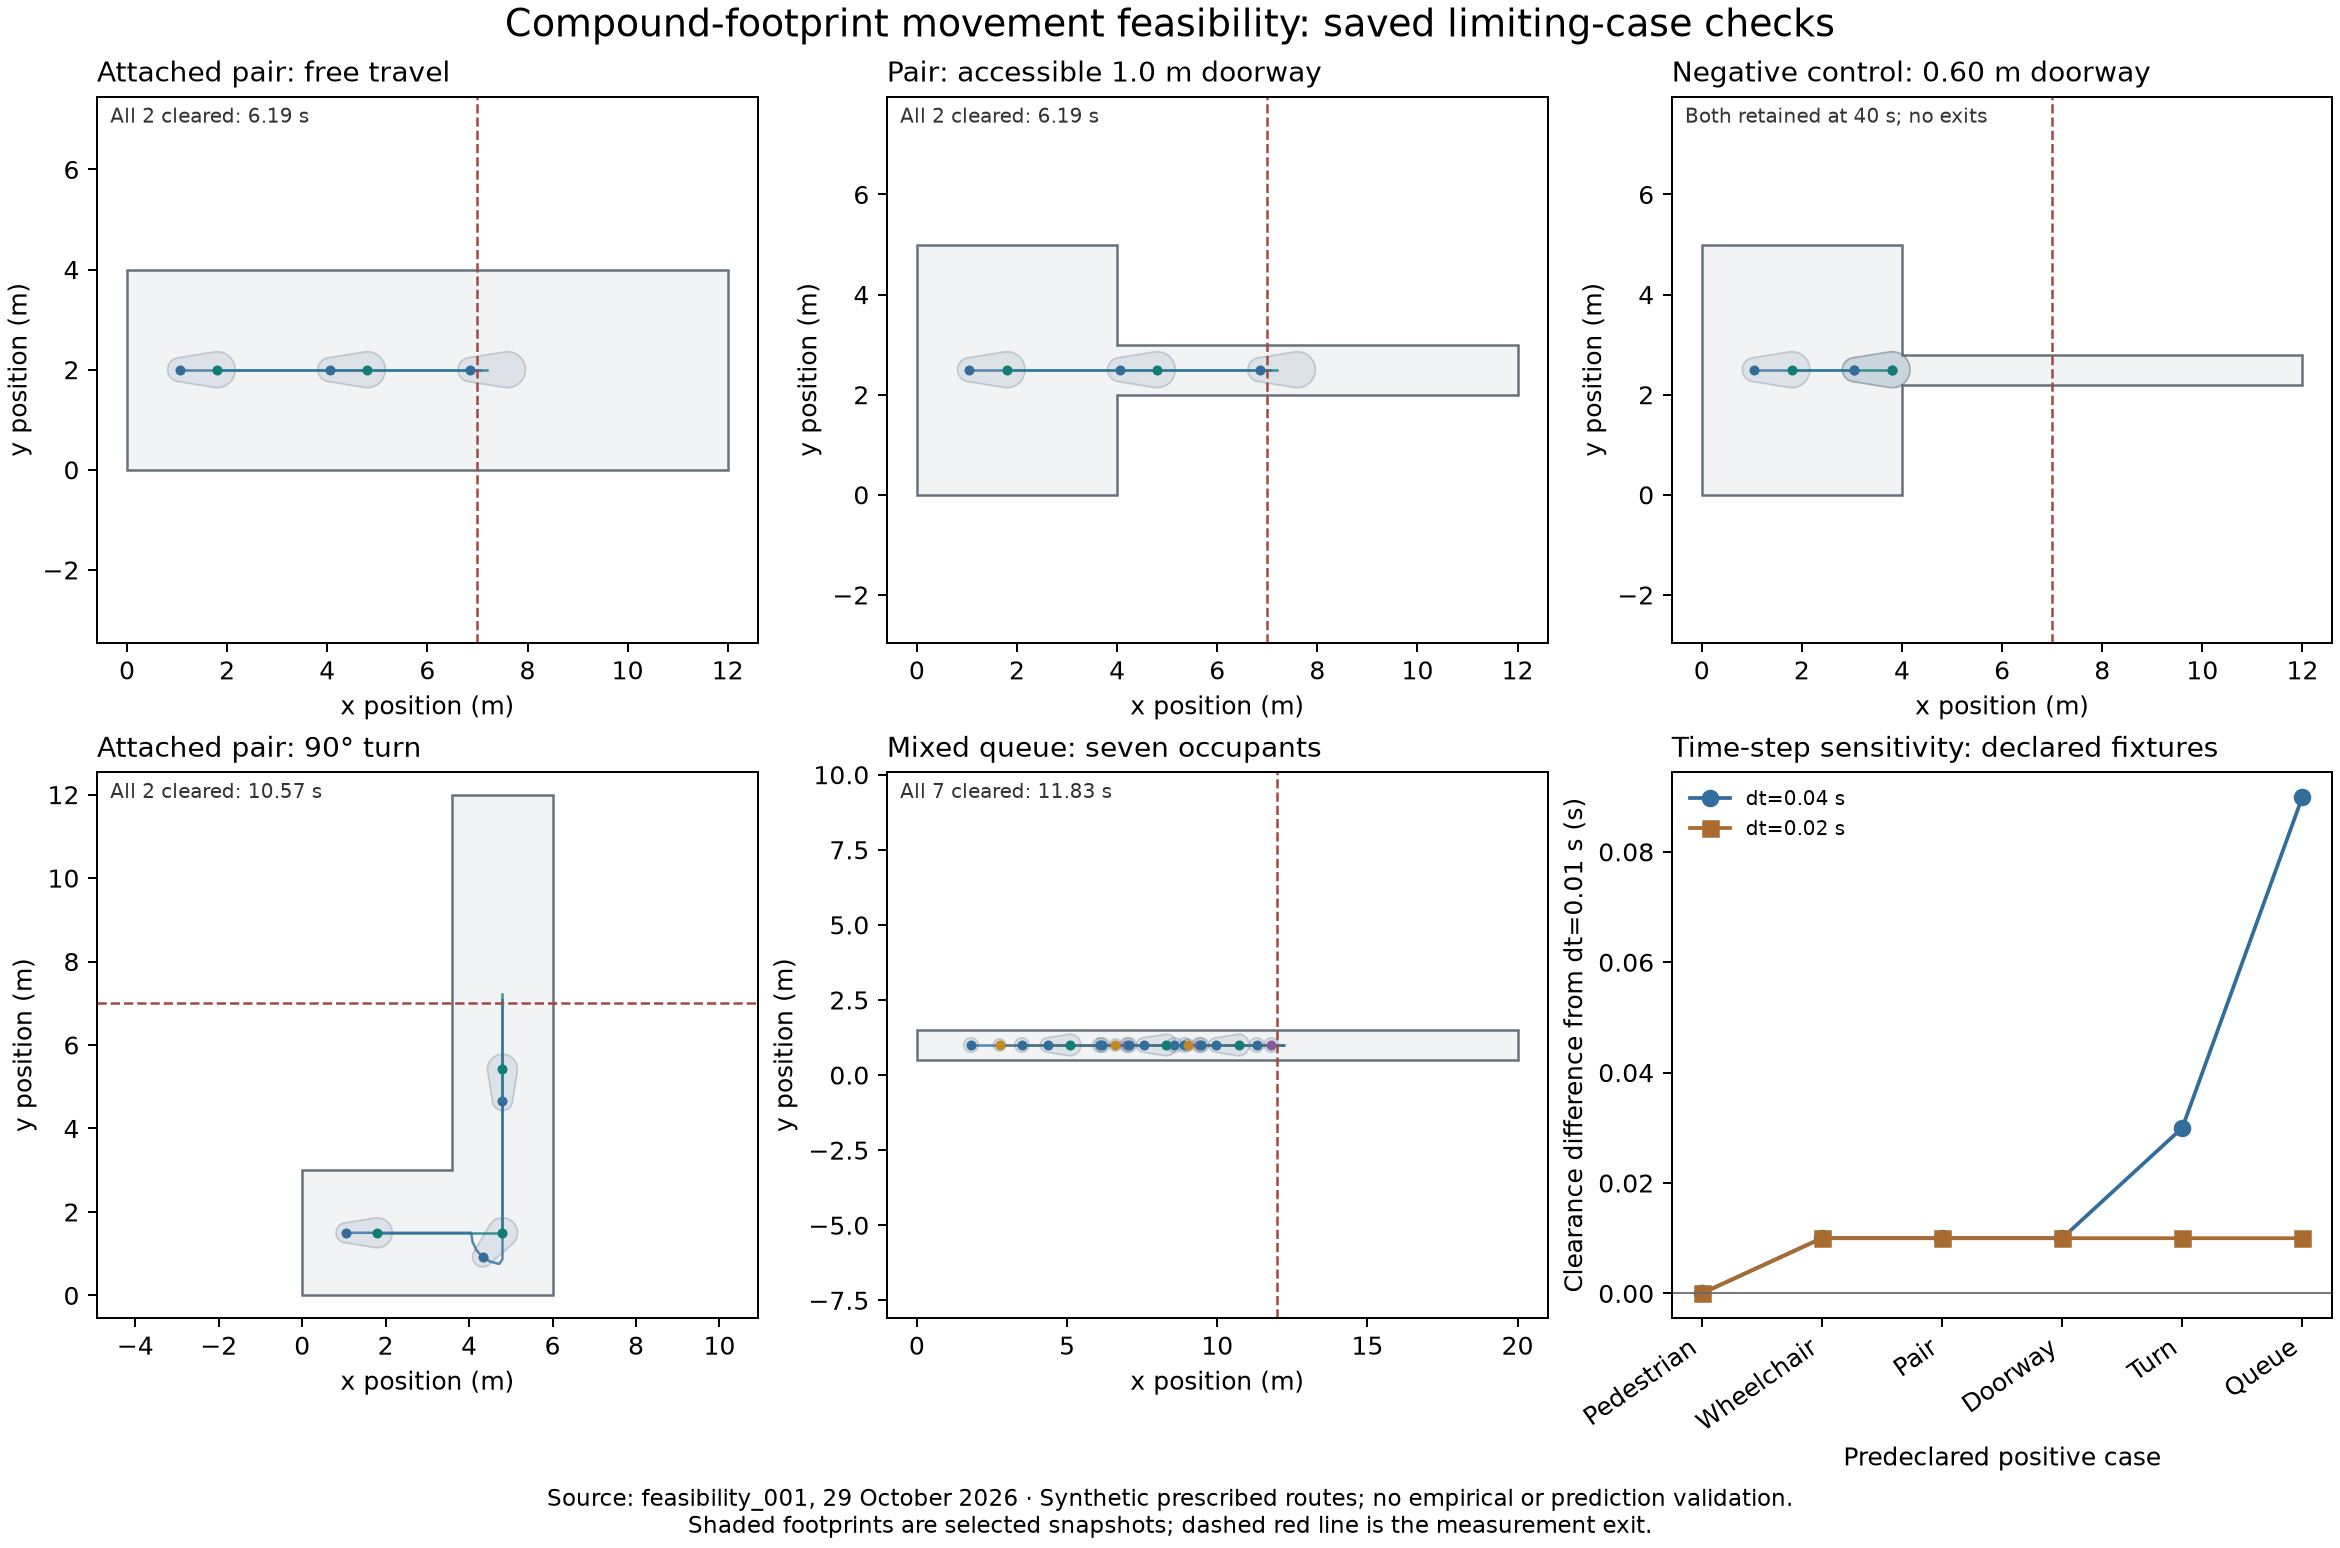
\includegraphics[width=0.94\textwidth]{images/movement_checks.png}
\caption{Saved movement verification: compound footprints reserve space while members retain separate identities. The narrow-door negative control retains the pair. Parameters and routes are synthetic; these fixtures are not human validation.}
\label{fig:movement}
\end{figure*}

\subsection{Populations, relationships and matched conditions}
N8 contains one reserved helper--wheelchair pair, one parent--child pair, two older-profile occupants and two additional adults. N12 contains two of each reserved pair, two older-profile occupants and two additional adults. Parents and helpers are distinct adults; each person is counted once. Uniform nominal speed ranges are adult 1.0--1.6, child 0.7--1.3, older 0.45--0.95 and wheelchair 0.55--1.05 m/s. Adult/older, child and wheelchair radii are 0.24, 0.20 and 0.36 m. These overlapping ranges are chosen experimental assumptions, not calibrated demographic norms.

Four conditions within each base block share capabilities, initial coordinates, queue order and latent draws: independent, family only, assistance only, and both. Family members remain separate collision units with commanded pace capped to the slower member's nominal pace. Active assistance units move at $\min(v_{\mathrm{helper}},g v_{\mathrm{client}})$, with $g\sim U[0.85,1.20]$. Assistance can therefore increase or decrease the client's unconstrained pace. Predictors do not receive $g$. Initial reserved-pair separation is 0.75 m, with 0.20 m clearance between queue blocks. All routes follow one centreline: overtaking, route choice, preparation delays and searching are absent. These mechanisms approximate shared pace and attachment rather than general family or assistance behaviour.

\subsection{Original design and causal inputs}
Table~\ref{tab:design} summarises the study partitions. The original main design crosses four corridor configurations, two population sizes, six seed slots and four conditions, producing 192 runs. G1/G2 are development configurations; G3/G4 are held out. Measurement lengths/widths are G1 18/1.0 m, G2 22/1.2 m, G3 20/0.9 m and G4 26/1.1 m. All have a 4 m outflow extension. Foremost initial centres lie at 10 m for N8 and 14 m for N12. New configurations change dimensions, not route topology.

\begin{table}[!t]\centering\small
\caption{Original frozen comparison. Four matched conditions form one base block. All checkpoints from a block stay in its partition.}
\label{tab:design}
\begin{tabular}{lrr}\toprule Partition or variant & Runs & Blocks\\\midrule
G1/G2 fitting, slots 0--2 & 48 & 12\\
G1/G2 validation, slot 3 & 16 & 4\\
G1/G2 same-corridor test, slots 4--5 & 32 & 8\\
G3/G4 held-out-configuration test & 96 & 24\\
Held-out support-gain counterparts & 32 & 8\\
Held-out finer-step counterparts & 16 & 4\\\bottomrule
\end{tabular}
\end{table}

Main trajectories use a 0.04 s time step, saved observations every 0.2 s, and 16 polygon segments per quadrant. Before held-out simulation or fitting, a prospective gate compared 16 development runs at 0.04/0.02 s. All completed; the maximum clearance difference was 0.08 s against the declared 0.5 s engineering criterion. Identical production-step pilots were reused with hash checks, not counted as additional samples. Thirty-two stress counterparts change $g$ to $U[0.70,1.40]$; sixteen use a 0.02 s step. Valid incomplete runs would retain the 180 s capped outcome rather than being silently excluded. Invalid accounting would stop production.

Queries occur at 2, 5 and 10 s. Inputs end at $t-0.2$ s; velocities use backward 0.2 s differences. Future frames/exits and centred smoothing are excluded. Queries are omitted only if completion is already observable at the cutoff. A uses 14 aggregate features: remaining count/density, speed summaries, slow fraction, distances to the exit, near-exit count, recent exits, elapsed time and dimensions. M adds 11 mobility features: profile fractions, exact nominal speed/radius summaries, minimum/rearmost nominal speed and mean/maximum nominal free-travel time. These queue-aware summaries constitute a strong reference; improvements cannot be attributed to age labels alone.

F adds nine link features: family/assistance counts per remaining occupant, pair distance and speed-difference summaries, helper-minus-client nominal-speed difference, and the fraction of assistance clients observed moving slowly. Edges contribute only while both endpoints remain in the permitted prefix. Exact nominal capabilities and relationships are supplied scenario information. Condition identifiers, seeds, private gains, computational grouping states and future outcomes are excluded. Hidden-parameter and future-frame invariance checks protect input construction.

\subsection{Learning and evaluation}
Each information set receives the same weighted linear ridge and RBF kernel-ridge search. Penalties are 0.01, 0.1 and 1, with RBF lengths 0.5, 1 and 2. For standardised vectors of dimension $d$, the kernel is
\begin{equation}
k(z_i,z_j)=\exp\!\left[-\frac{\|z_i-z_j\|^2}{2\ell^2d}\right].
\end{equation}
Scaling and kernel centring use fitting data only. Validation MAE selects settings, with fixed ties preferring ridge and then larger penalty/length. Models are refitted on fitting plus validation data; predictions are clipped to $[0,180-t]$. No held-out retuning occurs. Refitted ablations zero family or assistance columns. A counts-only model retains only the two link-count features beyond M. References include a fitting-weighted median and a validation-tuned count/width/capacity formula, not a comprehensive state-of-the-art benchmark.

For error $e_i=\hat y_i-y_i$, we report hierarchically weighted MAE, RMSE and mean underprediction:
\begin{align}
\MAE&=\sum_iw_i|e_i|, &
\operatorname{RMSE}&=\sqrt{\sum_iw_ie_i^2},\\
\operatorname{Under}&=\sum_iw_i\max(0,-e_i).
\end{align}
Weights average equally over queries within runs, four conditions within blocks, blocks within configurations, and configurations. Conditional descriptive 95\% intervals use 10,000 paired block-bootstrap draws within each fixed test configuration \cite{r6}. Models remain fixed; fitting, selection, generator and population uncertainty are excluded. Fixed-model link-removal/rewiring sensitivities preserve actual motion and outcomes. Repeated queries and matched conditions are not independent human participants.


\subsection{Exploratory Follow-up Design}
The negative original result motivated a broader learning comparison. Because its outcomes had been inspected, all 192 original main runs became development data. Slots 0--3 supplied 128 fitting runs/32 blocks; slots 4--5 supplied 64 validation runs/16 blocks across G1--G4. Entire blocks remained together. Settings, 18 fitted models, sources and fresh manifests were frozen before generating 144 new test trajectories.

The primary follow-up test contains 48 runs/12 blocks in G5 (24 m, 1.05 m) and G6 (28 m, 1.15 m). A secondary test contains 96 runs/24 blocks on G1--G4 using fresh seeds. SHA256-derived streams were checked against old seed collisions. The original movement engine and capability/gain distributions were unchanged. All 144 runs completed and all 432 queries were retained. These are fresh synthetic outcomes, not independent human observations.

Six families were fitted for A/M/F: linear ridge, RBF ridge, gradient boosting in scikit-learn 1.7.2 \cite{SKLEARN}, a small feed-forward MLP, a GRU in CPU PyTorch 2.7.1 \cite{TORCH}, and history-flattened ridge. Static learners see the last causal vector. GRU and history ridge see nine vectors over 1.6 s, ending at $t-0.2$ s; each historical vector uses its own lagged observations. History ridge distinguishes added temporal information from recurrent architecture. Dimensions remain 14/25/34 per vector; static and historical endpoints agree exactly.

Each family/information set receives three candidates. Ridge penalties are 0.01/0.1/1; RBF lengths are 0.5/1/2 at penalty 0.1. Boosting uses depths 1/2/3, 200 trees, learning rate 0.05 and minimum leaf count 8. MLP widths are 16/32/64; GRU hidden widths are 8/16/32. Neural candidates average three fixed seeds (113, 227, 331), each trained for 400 full-batch AdamW epochs at learning rate 0.003 and weight decay 0.01. Loss is weighted squared error on a training-standardised target. Input scaling uses training data only; selected settings/scalers are refitted on fitting plus validation data. There is no early stopping or best-seed selection.

Validation MAE selects both settings and the final family for each information set. The search contains 54 candidates, with equal candidate counts within each A/M/F family rather than equal computational budgets across architectures. All use identical labels, partitions, hierarchy and prediction clipping. The selected-system contrast may compare different families; family-matched results are therefore also reported. No test ranking is used to reselect a model.


\subsection{SiME Data and Reference-Replay Protocol}
A supplementary analysis uses public SiME trajectories \cite{SIME} to assess an unassisted reference model. It is separate from the compound simulator and does not validate the A/M/F forecasts. JuPedSim 1.4.2 CollisionFreeSpeedModelV2 implements a two-dimensional collision-free speed approach \cite{CFS} with recorded wall geometry. Observed first-forward crossings at $x=-6$ m supply inlet times and lateral positions; model interactions and pathfinding generate downstream crossings at $x=2.4$ m. Both observed and simulated head-centre crossings are interpolated between bracketing samples. These measured crossings, rather than an assumed evacuation formula, supply the empirical targets.

Future recorded inlets are supplied, making this conditional replay rather than an end-to-end forecast. Shared inlet times make downstream crossing error equal transit-time error. Alarm and pre-movement are absent; aggregate passage duration does not replace individual crossing accuracy.

Trials 1501/1507, with 0.9/1.2 m bottlenecks, provide development data. Eighteen desired-speed/radius/time-gap combinations are evaluated; thirteen complete both trials. Selection gives 1.6 m/s, 0.18 m and 1.0 s respectively, with development equal-trial crossing MAE 5.412 s. Failed completions remain in the trace. A documented head-to-body interface allows bounded lateral inlet conversion and delays admission when occupied, preserving identities. Frame-0 states are not projected into a fabricated complete cohort. Settings and source hashes are frozen before acquiring the two new test trials.

\section{Results}
\subsection{Original Frozen Comparison}
All 240 study runs completed and all 720 queries were retained. The audit verified trajectory hashes, occupant/exit accounting, circle separation and pair spacing over 31,143 sampled frames. Independent arithmetic reproduced all 32 model/evaluation groups. Fresh-process reproduction matched all 3,168 learned predictions within $6.84\times10^{-12}$ s. These are internal repeatability checks, not independent researcher replication.

\begin{table}[!t]\centering\small
\caption{Original held-out G3/G4 test: 96 runs, 24 matched blocks. All errors are seconds; lower is better.}
\label{tab:primary}
\begin{tabular}{lrrr}\toprule Predictor & MAE & RMSE & Under\\\midrule
Aggregate A & 2.660 & 3.001 & 0.304\\
Mobility M & 1.222 & 1.619 & 1.168\\
Full relationships F & 2.397 & 3.140 & 2.192\\
Counts-only & 1.235 & 1.629 & 1.182\\
Without family & 1.242 & 1.640 & 1.191\\
Without assistance & 1.233 & 1.629 & 1.177\\
Weighted median & 6.932 & 8.514 & 5.452\\
Tuned capacity & 7.795 & 9.560 & 4.973\\\bottomrule
\end{tabular}
\end{table}

M reduces primary MAE by 54.0\% relative to A (Table~\ref{tab:primary}). F increases error by 1.174 s relative to M: $\Delta=-1.174$ s, conditional interval $[-1.486,-0.882]$ s. The directional relationship-advantage hypothesis is not supported. This does not establish that relationships are generally irrelevant or accept a real-population null. Validation selected ridge for all learned models: penalty 0.01 for A, 0.1 for M and ablations, and 1 for F. Validation error already slightly favoured M (0.956 s) over F (1.001 s).

Counts-only and both ablations remain close to M, limiting a claim for detailed dyad summaries. Secondary M/F MAEs are 1.040/1.615 s on same-corridor tests, 1.062/1.968 s on gain-stress counterparts and 0.781/1.584 s on the finer-step subset. These subsets contain 8, 8 and 4 blocks respectively; differences between them do not isolate stress or resolution effects. Matched finer-step clearance differs by at most 0.16 s with unchanged completion status. This supports bounded sensitivity, not general convergence.

Removing one supplied link per available type yields F MAE 2.470 s; rewiring one per type yields 2.227 s versus 2.397 s intact. The apparently better rewiring can offset a poorly generalising fitted predictor; it does not validate incorrect metadata. As a post-result generator diagnostic, 40 of 48 family-only blocks and 19 of 48 assistance-only blocks have unchanged recorded last-exit time relative to independence. A slow occupant elsewhere can dominate a single-lane queue. Such matched clearance effects and forecast errors answer different questions.

\subsection{Exploratory Broader-Learner Results}
Figure~\ref{fig:learners} compares all six model families on both fresh synthetic tests; Table~\ref{tab:broad} gives the numerical results and conditional intervals.
\begin{figure*}[!t]\centering
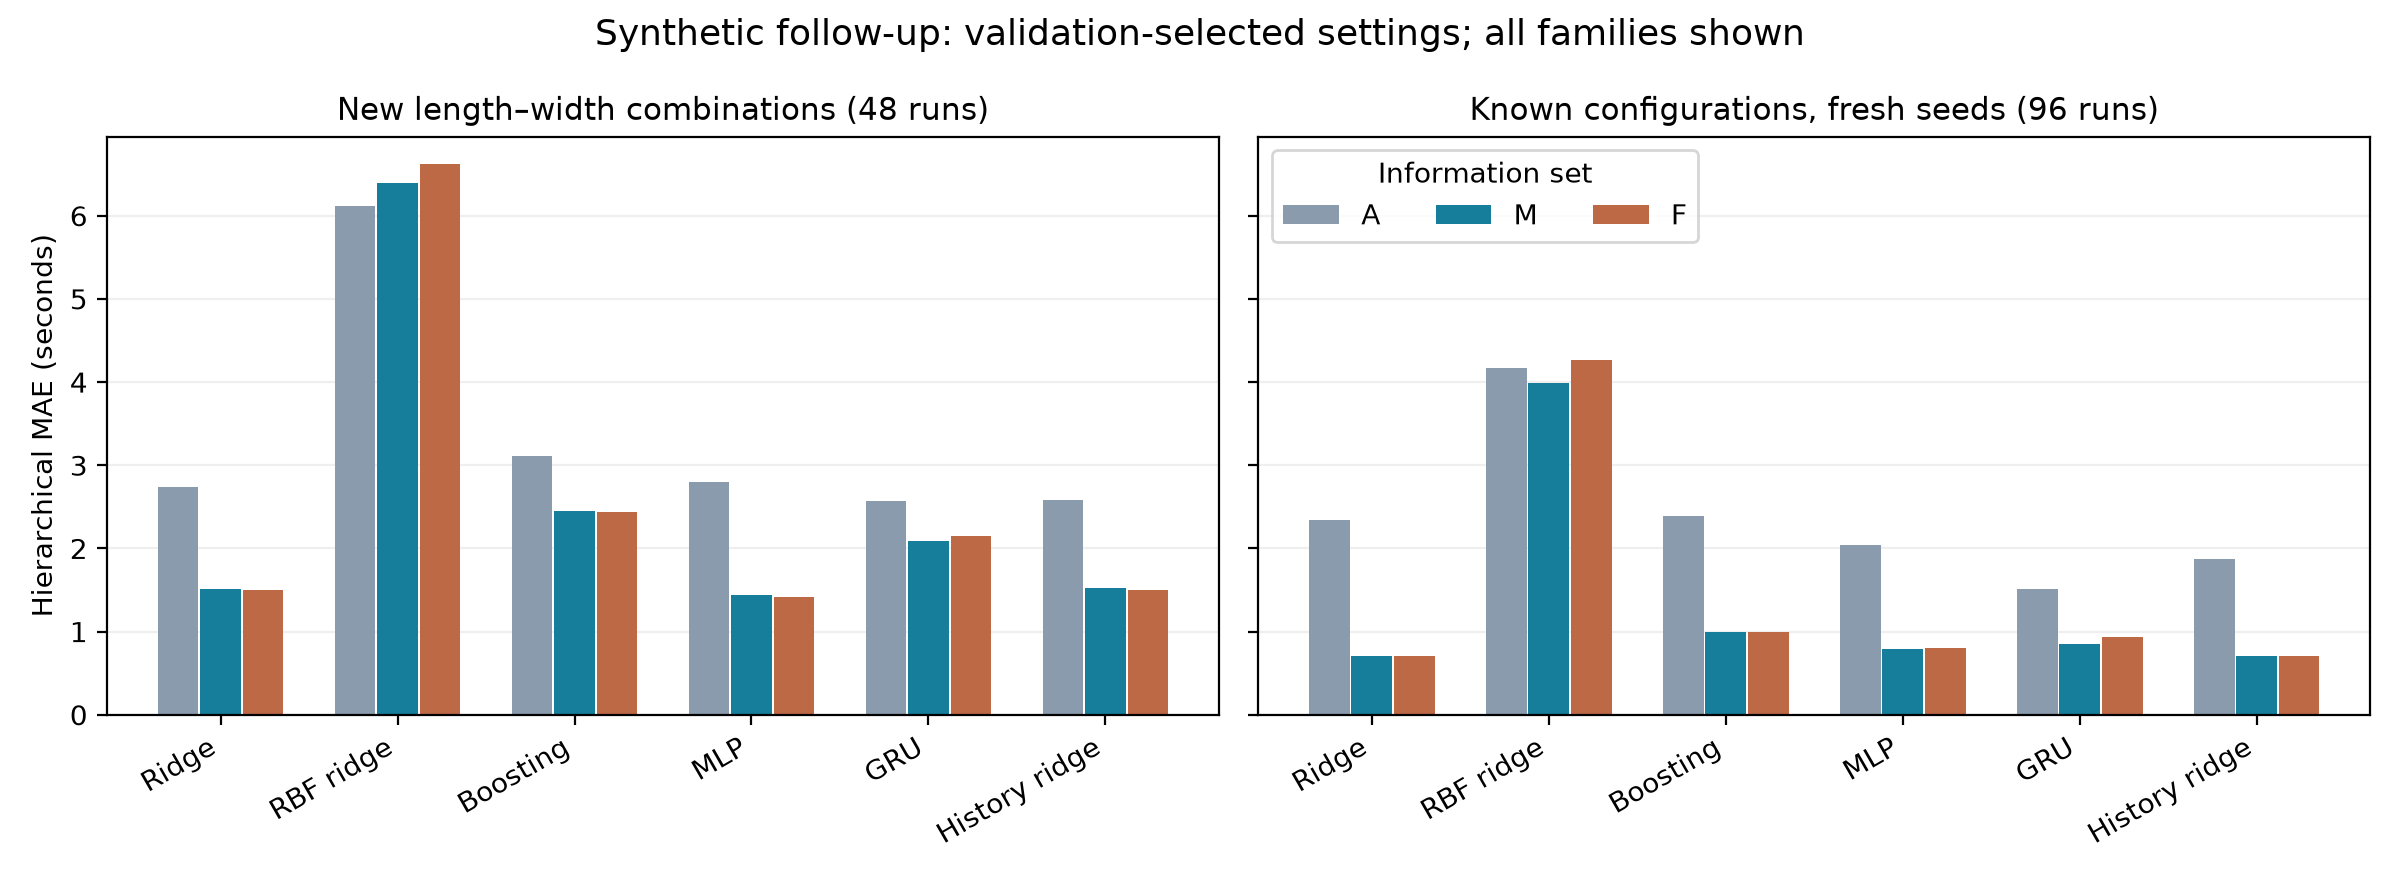
\includegraphics[width=\textwidth]{images/learner_comparison.png}
\caption{A/M/F mean absolute errors across six learning families. Lower is better. Settings were selected on development validation data and models were frozen before these fresh tests. GRU and history ridge use a short causal history; other families use the last vector.}
\label{fig:learners}
\end{figure*}
\begin{table*}[!t]\centering\small
\caption{Fresh synthetic tests under validation-selected settings. All values are seconds. New configurations contain 48 runs/12 blocks; fresh seeds on known configurations contain 96 runs/24 blocks. Positive $\Delta$ favours F. Intervals are conditional descriptive 95\% intervals, with fixed fitted models.}
\label{tab:broad}
\begin{tabular}{lrrrrlrrr}\toprule
&\multicolumn{5}{c}{New configurations: G5/G6}&\multicolumn{3}{c}{Known configurations, fresh seeds}\\
Learner & A MAE & M MAE & F MAE & $\Delta$ & Interval & A MAE & M MAE & F MAE\\\midrule
Ridge & 2.734 & 1.514 & 1.500 & $+0.014$ & $[-0.039,+0.080]$ & 2.341 & 0.703 & 0.705\\
RBF ridge & 6.123 & 6.395 & 6.621 & $-0.226$ & $[-0.351,-0.109]$ & 4.174 & 3.986 & 4.267\\
Boosting & 3.114 & 2.445 & 2.439 & $+0.005$ & $[-0.022,+0.039]$ & 2.386 & 0.991 & 0.998\\
MLP & 2.795 & 1.437 & 1.417 & $+0.020$ & $[-0.301,+0.343]$ & 2.037 & 0.785 & 0.798\\
GRU & 2.566 & 2.087 & 2.144 & $-0.057$ & $[-0.305,+0.211]$ & 1.516 & 0.854 & 0.938\\
History ridge & 2.584 & 1.529 & 1.498 & $+0.031$ & $[-0.025,+0.094]$ & 1.877 & 0.701 & 0.708\\\midrule
Validation-selected family & 2.584 & 1.437 & 1.500 & $-0.063$ & $[-0.380,+0.219]$ & 1.877 & 0.785 & 0.705\\\bottomrule
\end{tabular}
\end{table*}

Validation selects history ridge for A, MLP for M and ridge for F. On new configurations their MAEs are 2.584, 1.437 and 1.500 s, respectively (Table~\ref{tab:broad}). The selected-system contrast is $-0.063$ s, conditional interval $[-0.380,+0.219]$ s. On the secondary test, MAEs are 1.877/0.785/0.705 s and $\Delta=+0.081$ s, interval $[-0.100,+0.270]$ s. Both selected-system intervals span zero. F is slightly worse on new configurations and slightly better on known configurations with fresh seeds.

No family-matched interval wholly favours F. Several small positive point estimates on new configurations do not consistently recur on the secondary test. Boosting and GRU do not consistently exceed the simpler references within this bounded search. Independent standard-library MAE calculations agree within $8.9\times10^{-16}$ s, and all 18 persisted models reproduce predictions exactly in a fresh process. Source/model/trajectory hash, block-separation and input-causality checks pass.

\subsection{Held-out SiME Reference Replay}
\begin{table}[!t]\centering\small
\caption{Frozen SiME unassisted replay. MAEs are individual downstream crossing errors; passage is first-to-last downstream crossing duration. All times are seconds.}
\label{tab:sime}
\begin{tabular}{lrr}\toprule Measure & Trial 1503 & Trial 1505\\\midrule
Tracked person-trial records & 66 & 69\\
Replay crossing MAE & 5.343 & 4.129\\
Free-flight crossing MAE & 13.969 & 13.184\\
Observed passage & 46.850 & 43.358\\
Simulated passage & 52.767 & 45.788\\\bottomrule
\end{tabular}
\end{table}

The frozen test uses trials 1503/1505 at widths 1.0/1.1 m. All 135 person-trial records have contiguous-bracketed inlet/downstream targets, are admitted, cross and exit. Independent source-target reconstruction checks saved errors. Equal-trial crossing MAE is 4.736 s versus 13.576 s for a no-interaction free-flight reference under the same observed inlets: a 65.1\% reduction against that weak reference. The model nevertheless tends to predict later crossings. Table~\ref{tab:sime} separates individual error from overall passage duration. Trial/configuration separation does not prove independent participant cohorts.

At the finer 0.01 s step, equal-trial MAE becomes 5.583 s. Relative to 0.02 s, final crossing shifts by $-1.224$ s and $+3.098$ s in trials 1503 and 1505. No retuning occurs. These differences prevent a general convergence claim. Maximum sampled nominal-body wall penetration is 0.0282 m despite centre containment; sampled inter-agent overlap is zero. Neither this error magnitude nor improvement over free flight establishes a safety threshold.

Official device documentation and trajectory headers resolve seven wheelchair identities in each of two earlier inspected runs, but not assistant-track links or individual chronological ages. The reference replay has no disability, family or assistance controller. Qualitative assistance descriptions cannot become verified helper graphs, and wheelchair identities alone cannot validate the compound assistance mechanism. The replay supplies limited empirical evidence for a separate unassisted module while leaving the central transfer gap open.

\section{Discussion}
\subsection{What the comparisons establish}
The original comparison supports mobility information within the generator but not the directional relationship hypothesis. The broader search also finds no consistent incremental F value. A movement constraint can affect trajectories without changing the last exit or improving a fitted forecast; these findings do not imply that relationships never matter.

Exact capabilities and queue-aware summaries make M a strong reference. Correlated link features, limited validation diversity and configuration transfer may explain F's degradation, but their contributions are not isolated. The follow-up changes both development data and selected learners, preventing attribution of its smaller M/F gap to architecture alone.

Movement checks establish bounded geometric consistency; synthetic tests assess prediction under declared assumptions; SiME evaluates a different conditional movement replay. These evidence layers do not establish realistic rigid helper--wheelchair behaviour.

The follow-up is exploratory, with a bounded search and no multiplicity-adjusted population tests. Its conditional intervals exclude fitting, selection and generator uncertainty. Incremental relationship value remains inconclusive.

\subsection{External validity and statistical limitations}
Profiles are uncalibrated, populations contain 8/12 occupants, and forecasting routes share one centreline without overtaking. Turns are verification fixtures only. Rigid footprints omit steering, forces and realistic assistance mechanics; family rules omit searching and side-by-side movement. Preparation, discovery, attachment delays, multiple helpers and route choice are absent. Simulator exit times are implementation outcomes, not independently established human ground truth.

Exact capabilities and supplied links are strong assumptions. No video-based age, disability or relationship detector is evaluated; mobility improvement is not a causal age effect. Capability uncertainty, fatigue and helper misidentification require further study. SiME wheelchair identities lack verified helper mappings; proximity cannot supply those labels.

The original primary test has two configurations and four validation blocks; follow-up geometries change dimensions rather than topology. Queries and matched conditions are not independent participant cohorts. Fixed-model intervals omit population uncertainty. Three settings per family are not exhaustive optimisation. Historical screening provenance and an exhaustive novelty appraisal remain incomplete.

\section{Conclusion and Future Work}
This study separates verified movement implementation from incremental forecasting value. In the original frozen synthetic comparison, mobility reduces aggregate-reference MAE by 54.0\%, while full relationships increase error relative to mobility alone. A six-family exploratory follow-up on 144 fresh simulations leaves the relationship contrast small, inconsistent across test types and conditionally uncertain. The separate SiME replay improves on free flight under recorded inflows but does not validate assistance or end-to-end evacuation forecasts. The defensible contribution is an auditable matched evaluation and a bounded negative/inconclusive finding. Real assistance benefit, demographic realism and operational safety remain unresolved.

\subsection{Recommendations and Future Scope}
Retain a strong mobility-aware baseline, distinguish verification from human validation, and preserve negative findings. No operational evacuation decision or safety margin follows from these results.


Future work should first acquire compatible trajectories with measured inlet and exit crossings, individual mobility information and explicitly mapped helper--client roles. Capability and relationship estimates should include uncertainty rather than assume exact nominal speeds and perfect links. Nonrigid coordination, attachment delays, fatigue and family regrouping should be verified against observed behaviour before revised forecasting experiments.

Further tests should cover larger crowds, overtaking, turns, multiple exits and unseen route topologies. Relational or graph-based learners could then be compared with strong mobility and temporal baselines to test whether links help when interactions are more varied. Report both individual crossing errors and overall clearance, retain negative outcomes, and use fresh test data for any model revisions motivated by the present findings.

\section*{Research Declarations}
No external funding was received and no new participants were recruited. The reference replay reused public de-identified SiME trajectories; applicable institutional reuse requirements remain to be verified, and no new ethics approval is claimed. AI assistance supported coding, analysis and writing; the authors are responsible for verification.

\textit{Code and data availability:} Code, frozen protocols, synthetic trajectories and saved comparison outputs are retained in a private repository at \url{https://github.com/surya070/mobility-relationship-clearance}; access is by invitation. SiME source data are obtained from the original release cited in the paper.

